\documentclass[prb,12pt]{revtex4-2}

\usepackage{amsmath, amssymb,physics,amsfonts,amsthm}
\usepackage[most]{tcolorbox}
\usepackage{enumitem}
\usepackage{cancel}
\usepackage{booktabs}
\usepackage{polynom}
\usepackage{tabularx}
\usepackage{tikz}
\usepackage{hyperref}
\usepackage{enumitem}
\usepackage{ulem}
\usepackage{transparent}
\usepackage{caption}
\usepackage{float}
\usepackage{multirow}
\newtheorem{Theorem}{Theorem}
\newtheorem{Proposition}{Theorem}
\newtheorem{Lemma}[Theorem]{Lemma}
\newtheorem{Corollary}[Theorem]{Corollary}
\newtheorem{Example}[Theorem]{Example}
\newtheorem{Remark}[Theorem]{Remark}
\theoremstyle{definition}
\newtheorem{Problem}{Problem}
\theoremstyle{definition}
\newtheorem{Definition}[Theorem]{Definition}
\newenvironment{parts}{\begin{enumerate}[label=(\alph*)]}{\end{enumerate}}
%tikz
\usetikzlibrary{patterns}
\usetikzlibrary{matrix}
%tcolorbox
\tcbset{breakable=true,toprule at break = 0mm,bottomrule at break = 0mm}
% definitions of number sets
\newcommand{\N}{\mathbb{N}}
\newcommand{\R}{\mathbb{R}}
\newcommand{\Z}{\mathbb{Z}}
\newcommand{\Q}{\mathbb{Q}}
\newcommand{\C}{\mathbb{C}}
\allowdisplaybreaks
\setlength{\parindent}{0cm}
\captionsetup[table]{name=Tabelle}

\begin{document}
\title{Fortgeschrittene Fehlerrechnung Übungsblatt 4}
	\author{Jun Wei Tan}
	\email{jun-wei.tan@stud-mail.uni-wuerzburg.de}
	\affiliation{Julius-Maximilians-Universit\"{a}t W\"{u}rzburg}
	\date{\today}
	\maketitle
Die Regressionsparameter sind bestimmt durch
\begin{align*}
	a_1=&\frac 1\Delta \begin{vmatrix}
		\sum y_i \frac{1}{\sigma_i} & \sum \frac{x_i}{\sigma_i} & \sum \frac{x_i^2}{\sigma_i^2} \\ 
		\sum y_i \frac{x_i}{\sigma_i^2} & \sum \frac{x_i^2}{\sigma_i^2} & \sum \frac{x_i^3}{\sigma_i^2} \\
		\sum y_i \frac{x_i^2}{\sigma_i^2} & \sum \frac{x_i^3}{\sigma_i^2} & \sum \frac{x_i^4}{\sigma_i^2}
	\end{vmatrix}\\
a_2=&\frac 1\Delta \begin{vmatrix}
	\sum \frac{1}{\sigma_i^2} & \sum y_i \frac{1}{\sigma_i^2} & \sum \frac{x_i^2}{\sigma_i^2} \\
	\sum \frac{x_i}{\sigma_i^2} & \sum y_i \frac{x_i}{\sigma_i^2} & \sum \frac{x_i^3}{\sigma_i^2} \\
	\sum \frac{x_i^2}{\sigma_i^2} & \sum y_i\frac{x_i^2}{\sigma_i^2} & \sum \frac{x_i^4}{\sigma_i^2}
\end{vmatrix}\\
a_3=& \frac 1\Delta \begin{vmatrix}
	\sum \frac{1}{\sigma_i^2} & \sum\frac{x_i}{\sigma_i^2} & \sum y_i \frac{1}{\sigma_i^2}\\
	\sum \frac{x_i}{\sigma_i^2} & \sum\frac{x_i^2}{\sigma_i^2} & \sum y_i\frac{x_i}{\sigma_i^2} \\
	\sum \frac{x_i^2}{\sigma_i^2} & \sum \frac{x_i^3}{\sigma_i^2} & \sum y_i \frac{x_i^2}{\sigma_i^2}
\end{vmatrix}\\
\Delta=&\begin{vmatrix}
	\sum \frac{1}{\sigma_i^2} & \sum \frac{x_i}{\sigma_i^2} & \sum \frac{x_i^2}{\sigma_i^2} \\ \sum \frac{x_i}{\sigma_i^2} & \sum \frac{x_i^2}{\sigma_i^2} & \sum\frac{x_i^3}{\sigma_i^2} \\
	\sum \frac{x_i^2}{\sigma_i^2} & \sum \frac{x_i^3}{\sigma_i^2} & \sum\frac{x_i^4}{\sigma_i^2}
\end{vmatrix}
\end{align*}
\section{Herleitung des Fehlerausdrucks}
	Wir bestimmen $\sigma_{a_i}^2=\sum_k \left[\sigma_k \left(\pdv{a_i}{y_k}\right)^2\right]$. Dazu bestimmen wir zuerst $\pdv{a_i}{y_k}$. Weil
	\[\pdv{y_k}\sum_i y_i \frac{x_i^n}{\sigma_i^p}=\frac{x_k^n}{\sigma_k^p},\]
	können wir mit der Laplace-Entwicklung den Fehler berechnen
	\begin{align*}
		\frac{\partial a_1}{\partial y_k}=&\frac{1}{\Delta}\frac{1}{{\sigma_k}^2}\left[\sum \frac{{x_i}^2}{{\sigma_i}^2}\sum \frac{{x_i}^4}{{\sigma_i}^2}-\left(\sum \frac{{x_i}^3}{{\sigma_i}^2}\right)^2 
		- x_k\left(\sum \frac{{x_i}}{{\sigma_i}^2}\sum \frac{{x_i}^4}{{\sigma_i}^2}-\sum \frac{{x_i}^3}{{\sigma_i}^2}\sum \frac{{x_i}^2}{{\sigma_i}^2}\right)\right.\\
		&\left. +{x_k}^2\left(\sum \frac{{x_i}}{{\sigma_i}^2}\sum \frac{{x_i}^3}{{\sigma_i}^2}-\left(\sum \frac{{x_i}^2}{{\sigma_i}^2}\right)^2\right)\right]\\
		\frac{\partial a_2}{\partial y_k}=&\frac{1}{\Delta}\frac{1}{{\sigma_k}^2}\left[-\left(\sum \frac{{x_i}}{{\sigma_i}^2}\sum \frac{{x_i}^4}{{\sigma_i}^2}-\sum \frac{{x_i}^3}{{\sigma_i}^2}\sum \frac{{x_i}^2}{{\sigma_i}^2}\right)
		+ x_k\left(\sum \frac{1}{{\sigma_i}^2}\sum \frac{{x_i}^4}{{\sigma_i}^2}-\left(\sum \frac{{x_i}^2}{{\sigma_i}^2}\right)^2 \right)\right.\\
		&\left.-{x_k}^2\left(\sum \frac{{1}}{{\sigma_i}^2}\sum \frac{{x_i}^3}{{\sigma_i}^2}-\sum \frac{{x_i}^2}{{\sigma_i}^2}\sum \frac{{x_i}}{{\sigma_i}^2}\right)\right]\\
		\frac{\partial a_3}{\partial y_k}=&\frac{1}{\Delta}\frac{1}{{\sigma_k}^2}\left[\sum \frac{{x_i}}{{\sigma_i}^2}\sum \frac{{x_i}^3}{{\sigma_i}^2}-\left(\sum \frac{{x_i}^2}{{\sigma_i}^2}\right)^2 
		- x_k\left(\sum \frac{{1}}{{\sigma_i}^2}\sum \frac{{x_i}^3}{{\sigma_i}^2}-\sum \frac{{x_i}^2}{{\sigma_i}^2}\sum \frac{{x_i}}{{\sigma_i}^2}\right)\right.\\
		&\left.+{x_k}^2\left(\sum \frac{{1}}{{\sigma_i}^2}\sum \frac{{x_i}^2}{{\sigma_i}^2}-\left(\sum \frac{{x_i}}{{\sigma_i}^2}\right)^2\right)\right]\\
		\Delta&=\sum\frac{1}{{\sigma_i}^2}\left(\sum\frac{{x_i}^2}{{\sigma_i}^2}\sum \frac{{x_i}^4}{{\sigma_i}^2}-\left(\sum \frac{{x_i}^3}{{\sigma_i}^2}\right)^2\right) 
		- \sum\frac{{x_i}}{{\sigma_i}^2}\left(\sum \frac{{x_i}}{{\sigma_i}^2}\sum \frac{{x_i}^4}{{\sigma_i}^2}-\sum \frac{{x_i}^3}{{\sigma_i}^2}\sum \frac{{x_i}^2}{{\sigma_i}^2}\right)\\&+
		\sum\frac{{x_i}^2}{{\sigma_i}^2}\left(\sum \frac{{x_i}}{{\sigma_i}^2}\sum \frac{{x_i}^3}{{\sigma_i}^2}-\left(\sum \frac{{x_i}^2}{{\sigma_i}^2}\right)^2\right)
	\end{align*}
	Eingesetzt in ${\sigma_{a_i}}=\sqrt{\sum\limits_k\left[{\sigma_k}^2\left(\frac{\partial a_i}{\partial y_k}\right)^2\right]}$ liefert
	\begin{align*}
		&\sigma_{a_1}=\sqrt{\frac{1}{\Delta}\left(\sum \frac{{x_i}^2}{{\sigma_i}^2}\sum \frac{{x_i}^4}{{\sigma_i}^2}-\left(\sum \frac{{x_i}^3}{{\sigma_i}^2}\right)^2\right)}\\
		&\sigma_{a_2}=\sqrt{\frac{1}{\Delta}\left(\sum \frac{1}{{\sigma_i}^2}\sum \frac{{x_i}^4}{{\sigma_i}^2}-\left(\sum \frac{{x_i}^2}{{\sigma_i}^2}\right)^2\right)}\\
		&\sigma_{a_3}=\sqrt{\frac{1}{\Delta}\left(\sum \frac{1}{{\sigma_i}^2}\sum \frac{{x_i}^2}{{\sigma_i}^2}-\left(\sum \frac{{x_i}}{{\sigma_i}^2}\right)^2\right)}
	\end{align*}
\section{Polynomregression}
Die Daten sind in der Aufgabenstellung gegeben. Jede Bohrung entspricht 2,0 cm. Außerdem können wir ohne Beschränkung der Allgemeinheit die erste Bohrung als Ursprung ($y=0\text{ cm}$) definieren. Daraus berechnen wir die Datentabelle für die Regression

\begin{center}
	\begin{tabular}{ccc}
		\toprule
		\textbf{Bohrung} & \textbf{Zeit (s)} & \textbf{Ort (m)}\\\midrule
		1 & 0 & 0,00 \\\midrule
		2 & 0,065743 & 0,02 \\\midrule
		3 & 0,092204 & 0,04 \\\midrule
		4 & 0,111701 & 0,06 \\\midrule
		5 & 0,129847 & 0,08 \\\midrule
		6 & 0,143638 & 0,10 \\\midrule
		7 & 0,156868 & 0,12 \\\midrule
		8 & 0,169667 & 0,14 \\\midrule
		9 & 0,181285 & 0,16 \\\midrule
		10 & 0,192732 & 0,18 \\\midrule
		11 & 0,202532 & 0,20 \\\midrule
		12 & 0,21236 & 0,22 \\\midrule
		13 & 0,222212 & 0,24 \\\midrule
		14 & 0,230763 & 0,26 \\\midrule
		15 & 0,238582 & 0,28 \\\bottomrule
	\end{tabular}
\end{center}

Wir werden im Zukunft den Fehler durch die Streuung schätzen. Dann sind alle Fehler gleich und die $\sigma_i$ kürzen sich. Wir verwenden also eine alternative Definition von $\Delta$
\begin{align*}
	a_1=&\frac 1\Delta \begin{vmatrix}
		\sum y_i & \sum x_i & \sum x_i^2 \\ \sum y_i x_i & \sum x_i^2 & \sum x_i^3 \\
		\sum y_i x_i^2 & \sum x_i^3 & \sum x_i^4
	\end{vmatrix}\\
	a_2=&\frac 1\Delta \begin{vmatrix}
		N & \sum y_i & \sum x_i^2 \\ \sum x_i & \sum y_i x_i & \sum x_i^3 \\
		\sum x_i^2 & \sum y_i x_i^2 & \sum x_i^4
	\end{vmatrix}\\
	a_3=& \frac 1\Delta \begin{vmatrix}
		N & \sum x_i & \sum y_i \\
		\sum x_i & \sum x_i^2 & \sum y_i x_i \\
		\sum x_i^2 & \sum x_i^3 & \sum y_i x_i^2
	\end{vmatrix}\\
	\Delta=&\begin{vmatrix}
		N & \sum x_i & \sum x_i^2 \\ \sum x_i & \sum x_i^2 & \sum x_i^3 \\
		\sum x_i^2 & \sum x_i^3 & \sum x_i^4
	\end{vmatrix}
\end{align*}
Daraus ergibt sich
\begin{align*}
	\Delta=&0,0003341947203678026\text{ s}^{6}\\
	a_1=&0,00001890136308573145\text{ m}\\
	a_2=&-0,02499490722866542\text{ ms}^{-1}\\
	a_3=&4,997999358352541\text{ ms}^{-2}
\end{align*}

\begin{center}
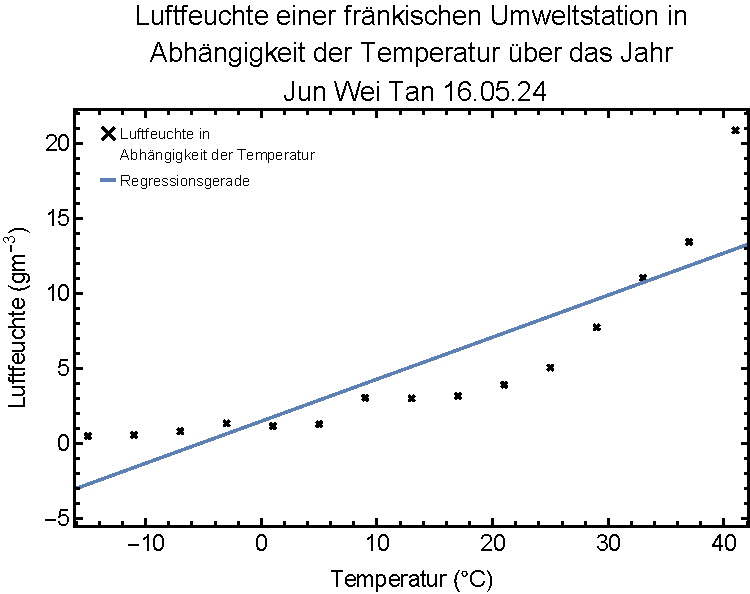
\includegraphics[width=0.75\textwidth]{plt.pdf}
\end{center}
\end{document}
